\documentclass[11pt,a4paper,sans]{moderncv}


\moderncvstyle{casual}                             
\moderncvcolor{blue}                              

\usepackage[utf8]{inputenc}
\usepackage[scale=0.75]{geometry}
\usepackage{graphicx}

\name{Valentina}{Del Rio Jimenez}
\phone[mobile]{3045230079}                   
\email{jimenezvalentina008@gmail.com}                        

\begin{document}

\recipient{Maquimas S.A.S}{Asunto: Devolución del dinero}
\date{15 de Octubre, 2025}
\opening{Respetados señores}
\closing{Atentamente,}
\enclosure[Anexos]{Anexo A:\@{}Comprobante de pago (imagen)}
\makelettertitle{}

Por medio de la presente, yo, Valentina del Río Jiménez, identificada con
cédula de ciudadanía No. \texttt{1041974771}, me permito informar que he
decidido no continuar con la negociación realizada con la entidad
\textit{Máquimas S.A.S.}, tras considerar que dicha operación no resulta
conveniente para mi situación personal y financiera.

En consecuencia, solicito de manera formal la devolución total del dinero
abonado como cuota inicial, correspondiente a la suma de un millón de pesos
($\$1.000.000$ COP), valor consignado a la fiducia administrada por su entidad,
conforme a las instrucciones previamente suministradas por \textit{Máquimas
    S.A.S.}

Solicito que la devolución se realice a la Cuenta de Ahorros No. 67800023538, a
nombre de \textit{Educational Corporation Building Happiness}, desde la cual se efectuó
el pago inicial.

Adjunto a la presente el comprobante de pago realizado, como soporte de la
transacción.

Adicionalmente, solicito se me expida un paz y salvo en el que conste que no se
llevó a cabo ningún tipo de negocio con \textit{Máquimas S.A.S.}, que no existe
vínculo contractual ni comercial vigente con dicha entidad, y que el valor
mencionado fue devuelto en su totalidad.

Finalmente, solicito que los datos personales suministrados durante el proceso
sean eliminados de sus sistemas, en cumplimiento de la Ley 1581 de 2012 y demás
normas relativas a la protección de datos personales.

Agradezco su atención y quedo atenta a una pronta respuesta.

\makeletterclosing{}

\clearpage{}
\section*{Anexos}
\addcontentsline{toc}{section}{Anexos}

\subsection*{Anexo A. Comprobante de pago}
Adjunto a la presente el comprobante del pago realizado (Anexo A)

\begin{center}
    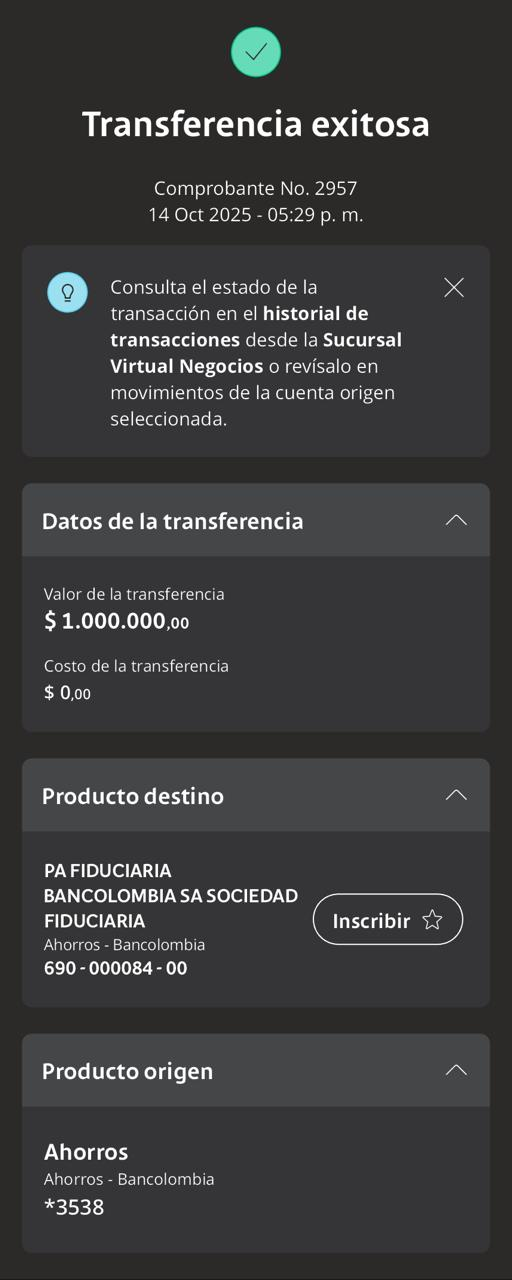
\includegraphics[width=0.45\textwidth]{comprobante.jpg}
\end{center}

\end{document}
